\subsection{Human Evaluation Tool}
\label{sec:humanevaltool}

In order to compare the performance of our page rank estimation model with humans, we have developed a basic evaluation tool. It allowed us to determine the accuracy of human individuals on the page rank task. Figure~\ref{fig:humanevalscreenshot} is a screenshot of the tool. The user opens the tool in their webbrowser and sees screenshots from two web pages. Then, the user can examine both of them and must decide which one they suspect to be ranked higher. After the decision, which can be expressed either by clicking onto the page or using the hotkeys, the tool shows the next tuple. A tuple may also be skipped, for instance if one of the pages is all-black. The pages are randomly chosen. The user can constantly see their accuracy and the number of samples they have assessed so far. Reloading the page will not result in loss, because the scores are saved in the browser's local storage. If desired, however, the score can be reset manually.

\begin{figure}\centering
    \makebox[\textwidth]{
        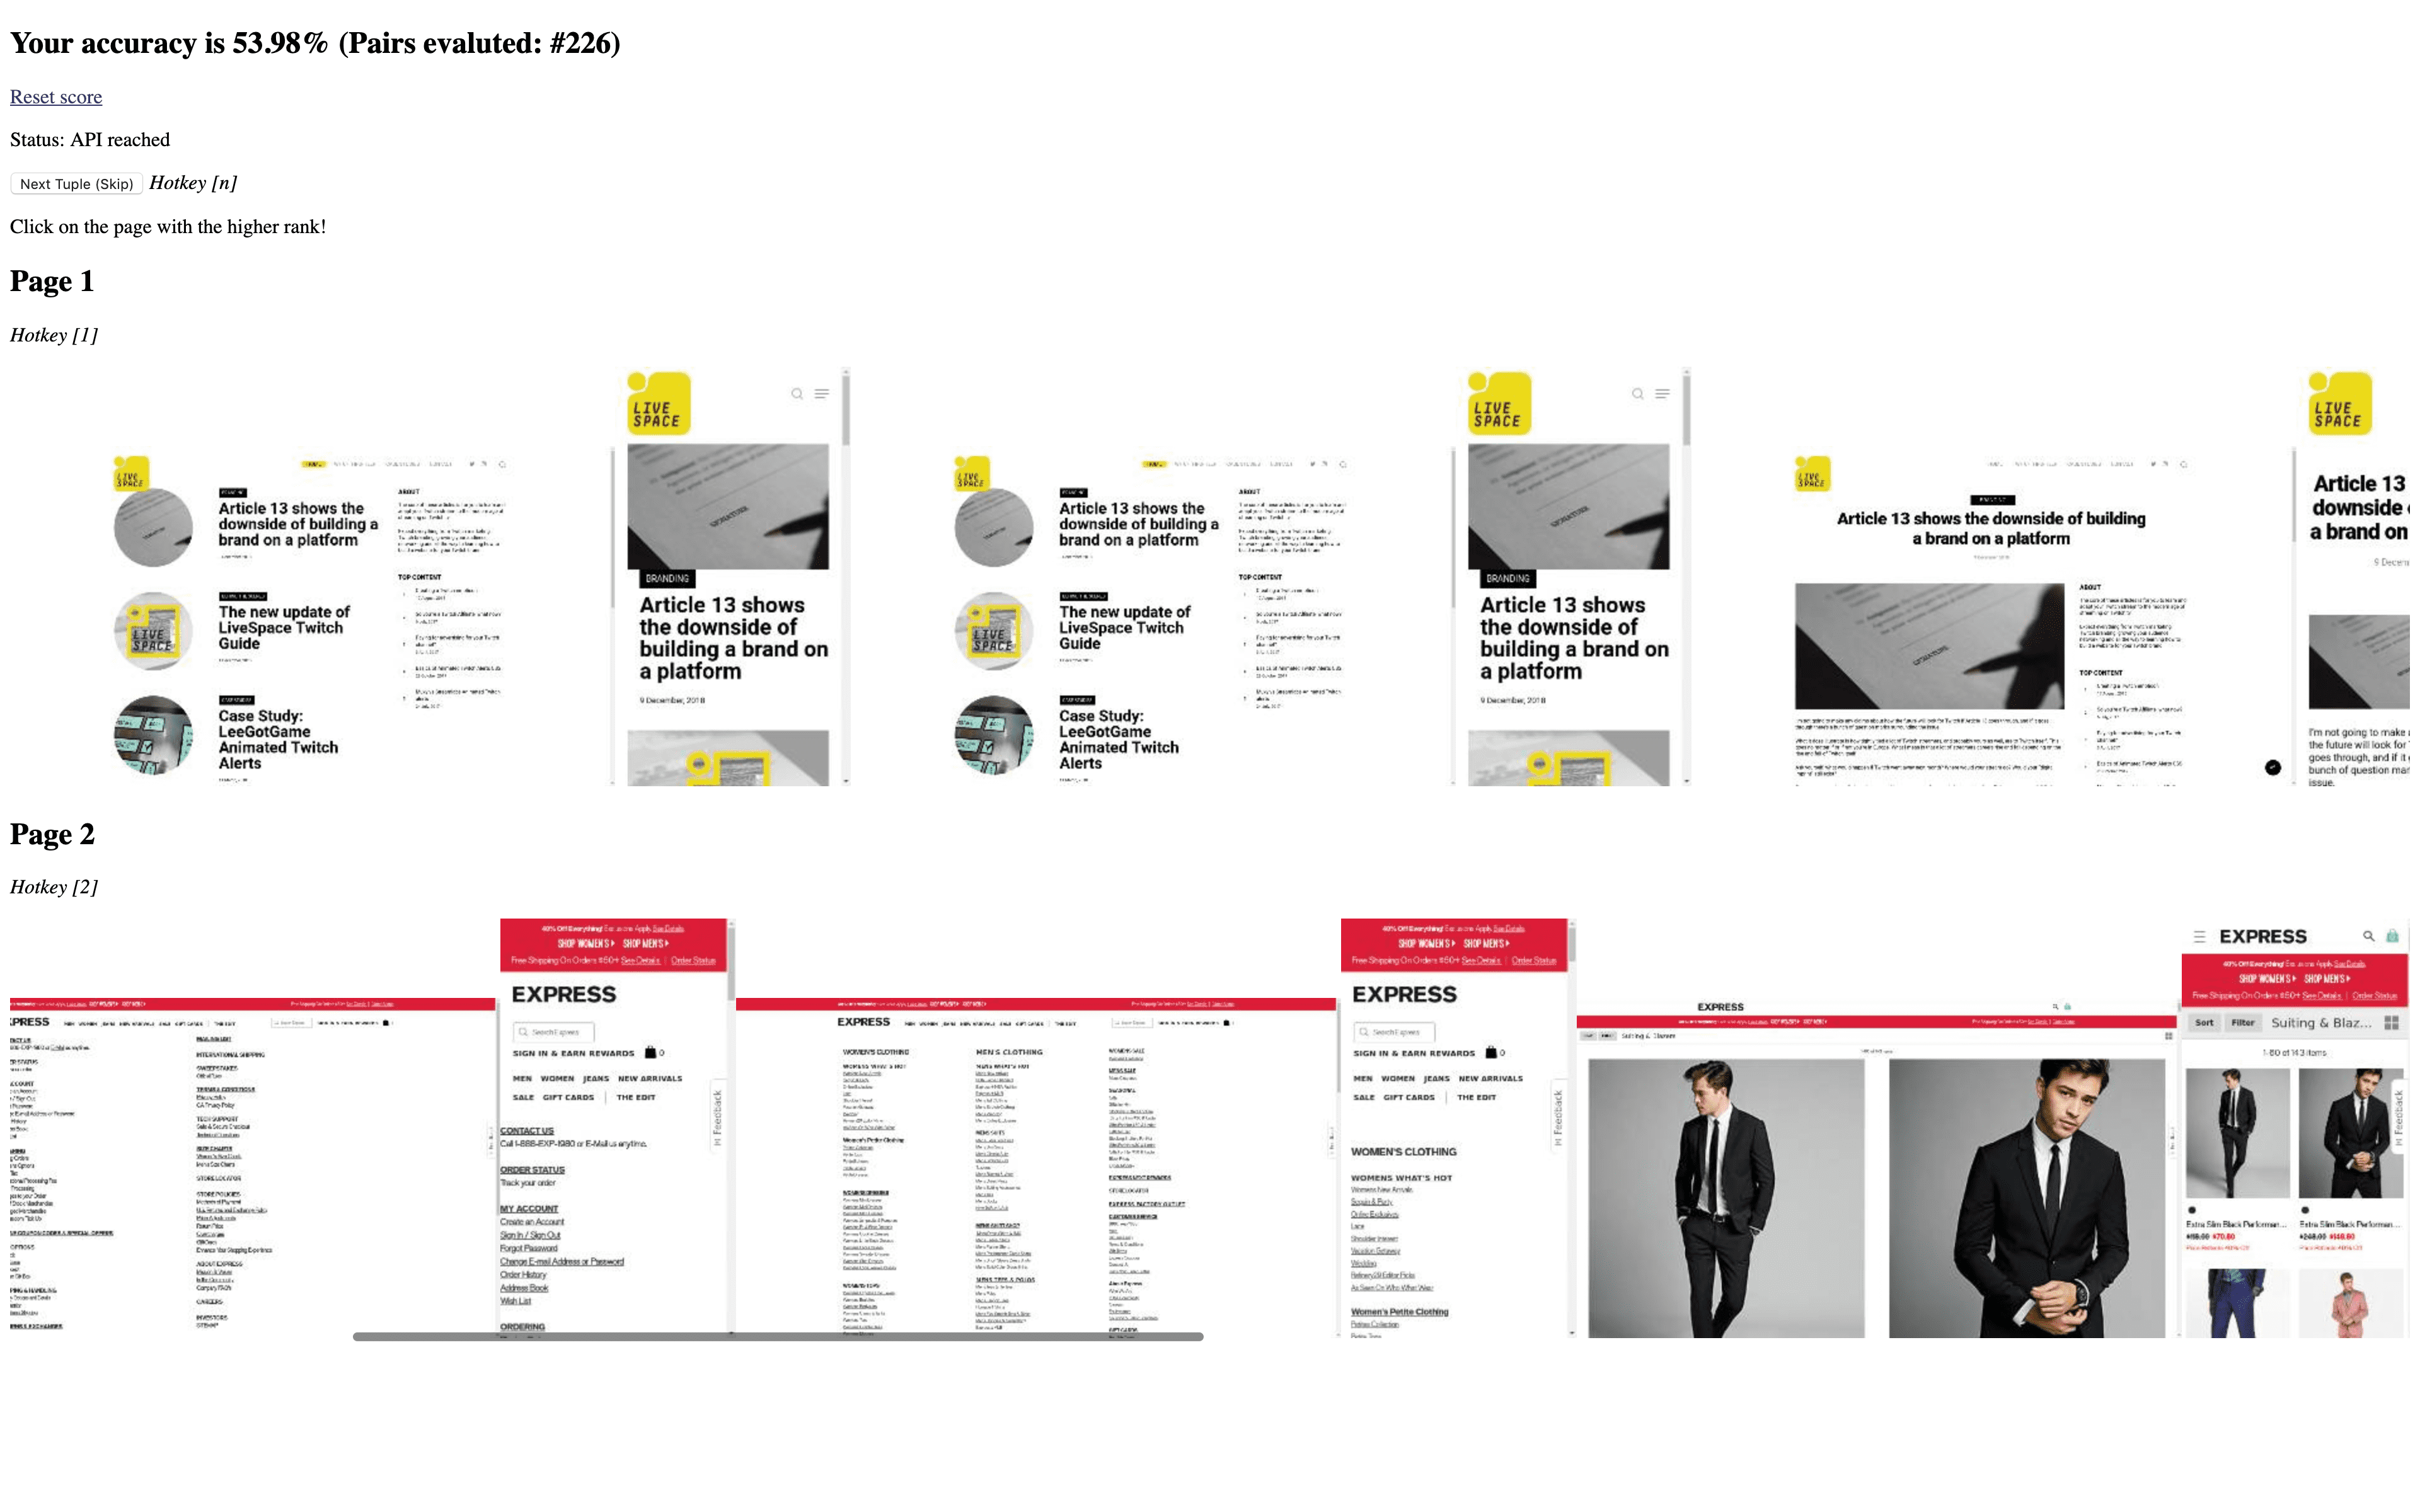
\includegraphics[width=\textwidth]{resources/human-eval-screenshot-min.png}
        }
    \caption[Screenshot of the human evaluation tool]{Screenshot of the human evaluation tool. The user has to decide which web page they expect to have a higher rank. What would your guess be? The page on top has the rank \#68,636, which is worse than \#15,898, the rank of the page below. Consequently, choosing the second page is correct, here.}\label{fig:humanevalscreenshot}
\end{figure}

The tool has a Node.js backend which provides an API. It serves the dataset images, meta information such as website ranks, and random tuples. The UI is very simple and has only few CSS styling rules.
